%!TEX root = ../thesis.tex
\section{General assumptions}

We consider a forager in two dimensions, searching for targets that are scattered throughout a boundaryless search space $\mathbb{R}^2$.
Targets are represented by points that are randomly distributed in the search space according to a homogeneous spatial Poisson point process.

We only consider destructive foraging in this \lcnamecref{sec:2dmodel}, since non-destructive foraging is more complicated.
%We discuss how non-destructive foraging may be investigated using this model in \cref{sec:conclusions}.
We discuss how non-destructive foraging may be investigated using this model in Chapter 7.

The forager begins its search at some point which we define to be the origin.
Each step in the forager's search strategy involves two parts.
Firstly, the forager selects a search direction, $\theta_i$, measured in radians about a unit circle centred at the current location.
Secondly, the forager selects a step length, $\ell_i$, in which to travel in the chosen direction. We can also define the \emph{turning angle}, $\beta_i:=\theta_i-\theta_{i-1}$, which is the change in direction from the previous step's direction, measured in radians.
The location of a forager after taking $i$ steps is then denoted as $(x_i,y_i)$.
The forager also has a constant radius of vision, $r_v$, and whenever a target is within this range the forager will be able to detect it and move directly towards it.
As a forager takes a step it can still detect targets while moving, and so each step will have an area of vision associated with it.

The possible search strategies that we consider are random walks with any choice of step-length distribution, and with uniform turning angles. 
Some extensions to the model are possible, such as allowing for arbitrary distributions for the turning angle, as well as considering Markov-modulated random walks, or even non-destructive targets,   although these may make the model intractable. 
We discuss some of these further in \cref{sec:conclusion}.

We begin by making a simplifying assumption: upon revisiting a previously explored area, a forager may still find targets within this area.
This is an equivalent scenario to the spatial Poisson process being redrawn in an already explored area, after a forager has already found it to be empty.
Under the simplest model, which we call the \emph{zeroth-order} approximation, the targets may have respawned in an area immediately following a search through that area.
Thus, a search that involved a lot of backtracking over the same area is not penalised for repeated searching of the same area.
In the \emph{first-order} approximation, the area covered in the previous step may not have food in it, although all area that was explored two or more steps ago may now have food. 
This means that the points within an explored area are redrawn, although with one step of lag.
This corresponds to some penalisation of backtracking, although not fully.

In general, the \emph{$n$th order} approximation means that a forager may not find food in any area already covered in the previous $n$ steps.
In the next section we solve the model analytically for both the zeroth-order and first-order models, and show why second-order and higher models are too complicated to consider analytically.
In \cref{sec:2dmodel:simulation}, we use simulations to model the same scenario, and can deduce the difference in results between different order approximations, including the case of no approximation ($\infty$-order).

As with the one-dimensional model, in two dimensions our primary aim is to determine the most efficient search strategy.
We maintain the same notion of efficiency as in the one-dimensional case. That is, the efficiency is defined as
\begin{equation}
\label{eq:2d:efficiency}
\eta = \frac{1}{\E{L}} ,
\end{equation}
where $L$ is the total distance travelled to find a target.
Based on the assumptions of our model we are able to show that this definition of efficiency is equivalent under the zeroth-order model to the efficiency as defined by Viswanathan \etal \cite{Viswanathan_1999}, which is
\begin{equation}
\label{eq:2d:vis_efficiency}
\eta = \frac{1}{\E{\abs{\ell}} \E{N}},
\end{equation}
where $\E{\abs{\ell}}$ is the expected distance travelled in a single step, and $\E{N}$ is the expected number of steps to find a target.

Due to the complete spatial randomness of the target distribution, we can make a few simplifications to the model.
The probability of a target being within some searched area depends on the size of the area and the density of the targets.
Since the targets have a homogeneous spatial Poisson distribution, the density is constant everywhere.
This means that the start and end locations of a step make no difference to the probability of finding food, and what really matters is the search area covered by a step.
Thus, we do not actually need to keep track of the forager's location, and can without loss of generality assume that each step begins at the origin.
For the first-order approximation, we do need to track the search area of the previous step and determine the overlapping area between that and the current step.

We make one final assumption; that there are no targets within the initial radius of vision of the forager before taking any steps.
This is reasonable since if there was, a forager would immediately move to this food target and then begin searching again, repeating this process until there was no target within its initial radius of vision.

\iffalse
\begin{figure}
	\begin{center}
		\begin{tikzpicture}
		\filldraw[black] (0,0) circle (2pt) node[anchor=north west] {$(x_i,y_i)$};
		
		\draw[black] (-2,2) circle (1);
		\filldraw[black] (-2,2) circle (2pt); 
		\draw[black](-2,2) -- (-1,2) node[anchor=north east] {$r_v$};
		
		\draw[black] (3,-1) circle (1);
		\filldraw[black] (3,-1) circle (2pt); 
		\draw[black](3,-1) -- (4,-1) node[anchor=north east] {$r_v$};
		
		\draw[black] (3.5,3) circle (1);
		\filldraw[black] (3.5,3) circle (2pt); 
		\draw[black](3.5,3) -- (4.5,3) node[anchor=north east] {$r_v$};
		\end{tikzpicture}
		\caption{Example layout for two-dimensional search model. targets are represented by points, and are spread out about the search space. The forager's radius of vision is represented by the circles around the targets, within which the forager can locate the food.  \label{fig:2dtargets}}
	\end{center}
\end{figure}
\fi



\section{Solving the model analytically}

In deriving an analytic expression for the efficiency, much of the process depends on the order of model we are considering. We initially begin deriving expressions for the probability of finding a target on any given step, and for the expected length of a single step, for any order of model. Then, in \cref{sec:2dmodel:0thorder} we use these expressions to find an analytic expression for the efficiency for the zeroth-order model. In \cref{sec:2d:1storder}, we consider the first-order model, and are unable to derive an exact expression for the efficiency, and we discuss why this is the case.

In \cref{sec:1dRW} we found an expression for the total cost to find a single target, which we simplified in \cref{eq:1dRW_cost:Q_rearranged} to
\begin{equation*}
Q(x_0) = \sum_{n=0}^{\infty} \indic_{(\tau \geq n+1)} q(X_n,X_{n+1}),
\end{equation*}
where $Q(x_0)$ was the total cost for a search beginning at $x_0$, and $q(X_n,X_{n+1})$ was the cost attributed to a step that begins at $X_n$ and ends at $X_{n+1}$, and the random variable $\tau$ represented the time until food was found. In the case of our two-dimensional model, we are not interested in finding a general cost function, but rather, the total length travelled to find food. Thus, we get
\begin{equation*}
L = \sum_{n=0}^\infty \indic_{(\tau \geq n+1)} \abs{\ell (X_n,X_{n+1})},
\end{equation*}
where we can also drop the dependence on the starting location $x_0$, since all starting locations are considered equivalent. 
\begin{equation*}
\E{L} = \sum_{n=0}^\infty \E{ \indic_{(\tau \geq n+1)} \abs{\ell_n (X_n,X_{n+1})}},
\end{equation*}
which we can rewrite as
\begin{equation*}
\E{L} = \sum_{n=0}^\infty \E{ \abs{\ell (X_n,X_{n+1})} \mid \indic_{(\tau \geq n+1)}} \Pr(\tau \geq n+1).
\end{equation*}
Since our step-length distribution has no dependence on the start or end locations, we may rewrite this without the dependence on $X_n$ and $X_{n+1}$. However, we include a subscript on the $\ell$ to denote the step number, since for first-order and higher models we need to keep the step number in mind. 
Thus,
\begin{equation*}
\E{L} = \sum_{n=1}^\infty \E{ \abs{\ell_n } } \Pr(\tau \geq n).
\end{equation*}
where we have also shifted the summation. 
Thus, we now have two expressions --- the expected length of a single step, and the probability that food is located within $n$ steps --- that must be found in order to solve for the efficiency. 

Both of these expressions will depend on whether we are considering the zeroth-order or the first-order approximation. Since the targets have a homogeneous spatial Poisson distribution, the starting point of a step will not affect the probability that food is located. The probability of finding exactly $k$ points within productive area $a$, with food density $\rho$, is
\begin{equation*}
\Pr(k,\rho,a) = \frac{(a\rho)^k e^{-(a\rho)}}{k!}.
\end{equation*}
Let $f_A(a)$ represent the \ac{PDF} of the area covered in a single step. The probability of not finding a target on a given step is then
\begin{align}
\Pr(\text{not found}) &= \int_{A_{\min}}^\infty \Pr \left( \text{not found} \mid A=a\right) f_A(a)da \nonumber \\ 
&=\int_{A_{\min}}^\infty\Pr(0,\rho,a)f_A(a)da \nonumber \\
&=\int_{A_{\min}}^\infty e^{-a\rho} f_A(a)da. \label{eq:2d_prob_not_found}
\end{align}
Therefore, the probability of finding a target on any given step is
\begin{equation}
\label{eq:2d_prob_found}
\Pr(\text{found}) = 1 - \int_{A_{\min}}^\infty e^{-a\rho} f_A(a)da.
\end{equation}
We use \cref{eq:2d_prob_found} to solve for $\E{N}$, although how we now proceed depends on which order of the model we are considering. We derive $\E{N}$ for the zeroth-order model in \cref{sec:2dmodel:0thorder}.

Next, we derive an expression for the expected length of a single step that is valid for any order of model. This expression is similar to the expectation of the step-length distribution, except we must take into account the possibility of a step being truncated:
\begin{equation}
\label{eq:2d_El}
\E{\abs{\ell}} = \int_{\lmin}^\infty \E{\ell_T \mid \ell} f(\ell)d\ell,
\end{equation}
where $\E{\ell_T \mid \ell}$ is the expected truncated length of a step which would have had full length $\ell$. Let $A(u,\beta)$ represent the new area covered by a step of length $u$ and with turning-angle $\beta$. Since the targets are distributed according to an homogeneous spatial Poisson process, the probability of finding a target after moving certain distance is exponentially distributed with parameter $\rho A(u,\beta)$. Then, the truncated length will be given by
\begin{equation}
\label{eq:2d_El_split}
\E{\ell_T \mid \ell} = \int_{\beta=0}^{2 \pi}\int_{u = 0}^{\ell} \rho A(u,\beta) e^{- \rho A(u,\beta)} \frac{1}{2\pi}  du d\beta +  \ell \int_{\beta=0}^{2 \pi}  \left(e^{-\rho A(u,\beta)}\right) \frac{1}{2\pi}  d\beta,
\end{equation}
where the first term represents when the forager finds a target, and hence truncates the distance to $u$, whereas for the second integral the target is not found and the forager travels a full distance $\ell$. The $1/(2\pi)$ in both terms comes from the distribution of the turning angle, which is uniform between $0$ and $2 \pi$. Note also that the integral does not begin at $\lmin$ but rather at $0$ since a step may be truncated after less than $\lmin$ has been travelled. To solve this further we need an expression for $A(u,\beta)$, which depends on which order approximation we are considering.


\subsection{Zeroth-order approximation}
\label{sec:2dmodel:0thorder}


To solve for the efficiency of the zeroth-order approximation, we first need an expression for the amount of new area travelled, $A(\ell,\beta)$, for a step of length $\ell$, and a turning-angle $\beta$. Consider a single step of a forager's search, where the forager begins at a point that is not within vision range of a target. While travelling a distance $\ell$, the forager can see $ r_v$ distance around itself in all directions, which results in a rectangular shaped area (of dimension $2 r_v$ by $\ell$) that is searched while travelling. Once landing, the forager can also see $r_v$ in all directions around itself, resulting in a circle shaped area of searching (with radius $r_v$). We do not need to include the initial circle of radius $r_v$ since this cannot have a target in since the previous step did not find food. As mentioned earlier, we can without loss of generality assume that this circle on the initial step does not contain food, as if it did, the forager immediately finds and destroys it, and the search begins again at this new origin. The overlap between these three regions must also be accounted for, to avoid double counting some of the area. \cref{fig:2dbless:searcharea} shows the area in question, which totals
\begin{equation*}
\label{eq:2dbless:searcharea}
A(\ell,\beta) = 2\ell r_v - \frac{1}{2}\pi r_v^2 + \frac{1}{2} \pi r_v^2 = 2\ell r_v,
\end{equation*}
and is therefore not a function of the turning-angle. Further, we can approximate the area searched in each step by a forager as a rectangle, which for the zeroth-order model is still $A(\ell,\beta) = 2\ell r_v$, as in \cref{fig:2dbless:searcharea_rectangle}.
\begin{figure}
	\centering[H]
	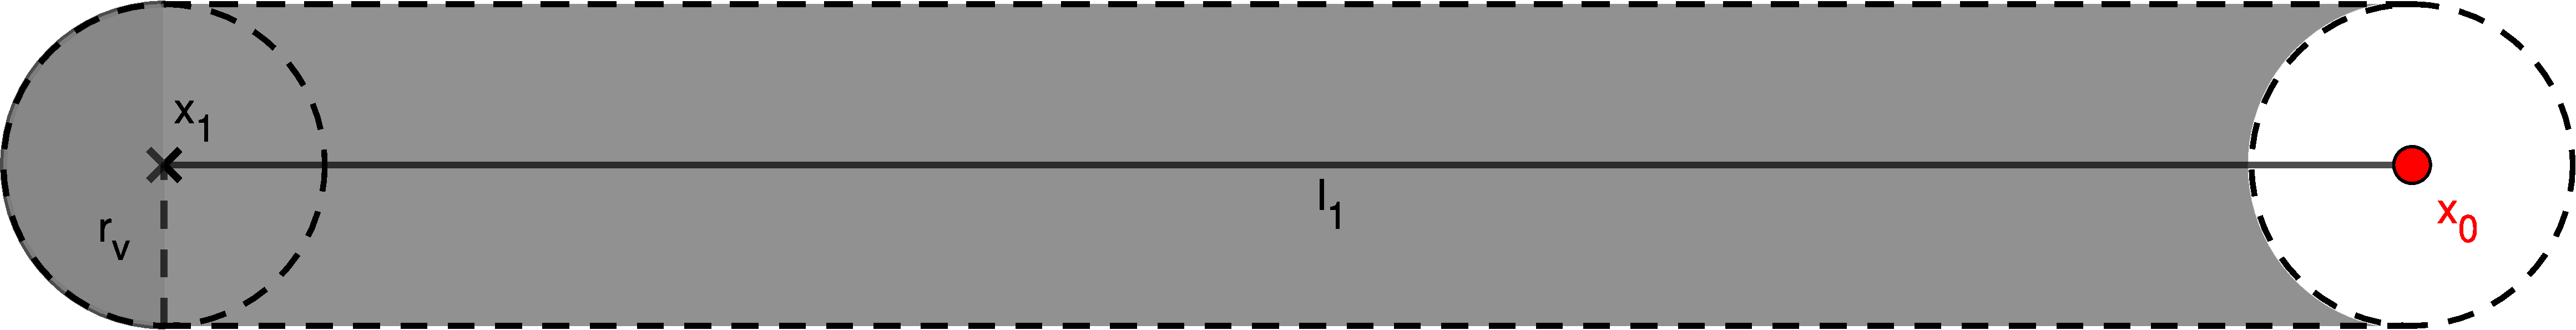
\includegraphics[width=1.0\textwidth]{2D-0thOrderApproximation-crop}
	\caption[Area covered by a step in the zeroth-order model]{A step from location $x_0$ to $x_1$. The search area that is explored by the forager is shaded in grey. The initial circle of radius $r_v$ around the forager is known to be empty, otherwise the forager's search would have ended during the previous step. \label{fig:2dbless:searcharea}}
\end{figure}

\begin{figure}[h!]
	\centering
	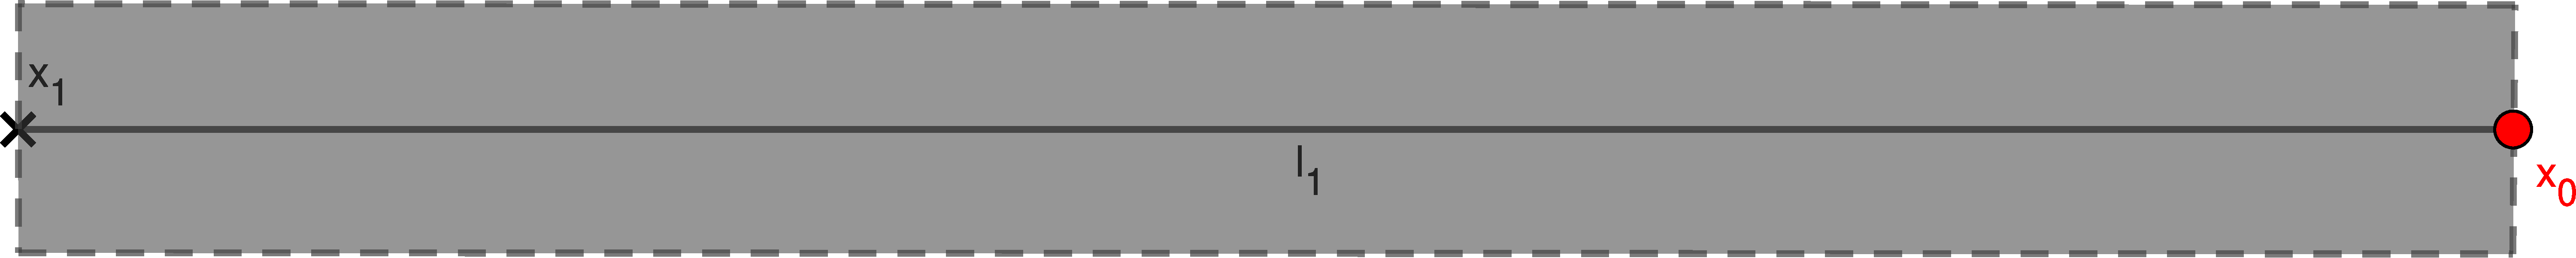
\includegraphics[width=1.0\textwidth]{2D-0thOrderApproximation_rectangles-crop}
	\caption[Area covered by a step in the zeroth-order model, simplified into a rectangle]{A step from location $x_0$ to $x_1$. The search area that is explored by the forager is shaded in grey, and has now been simplified into a rectangle by not taking into account the radius of vision around the forager at either end of a step. The total area is still the same. \label{fig:2dbless:searcharea_rectangle}}
\end{figure}



Since $\ell$ is a random variable, $A$ is also a random variable, which in our case is
\begin{equation*}
f_A(a) = \frac{f\left( \frac{a}{2r_v}\right)}{2r_v}.
\end{equation*}
The probability of not finding food, from \cref{eq:2d_prob_not_found}, was
\begin{align*}
\Pr(\text{not found}) &=\int_{A_{\min}}^\infty e^{-a\rho} f_A(a)da\\
& =\int_{A_{\min}}^\infty \frac{e^{-2r_v\ell\rho}}{2r_v} f\left(\frac{\ell}{2r_v}\right)d\ell,
\end{align*}
for which integration by substitution yields
\begin{equation}
\label{eq:2dbless:not_found_prob}
\Pr\left(\text{not found}\right) = \int_{\lmin}^\infty e^{-2 \ell r_v \rho} f(\ell)d\ell,
\end{equation}
which can now be solved exactly, depending on the step-length distribution.

Since the probability of finding food is the same for every step under our zeroth-order model, we can consider $\tau$ as a geometric random variable. 
 
The fact that $\tau$ is geometrically distributed also tells us that the expectation of the total number of steps is
\begin{equation}
\label{eq:2d_model:EN}
\E{N} = \frac{1}{\Pr(\text{found})} = \left( 1-  \int_{\lmin}^\infty e^{-2 r_v \ell \rho} f(\ell)d\ell \right)^{-1},
\end{equation}
which is used in evaluating the efficiency.

Recall \cref{eq:2d_El_split}, 
\begin{equation*}
\E{\ell_T \mid \ell} = \int_{\beta=0}^{2 \pi}\int_{u = 0}^{\ell} \rho A(u,\beta) e^{- \rho A(u,\beta)} \frac{1}{2\pi}  du d\beta +  \ell \int_{\beta=0}^{2 \pi}  \left(e^{-\rho A(u,\beta)}\right) \frac{1}{2\pi}  d\beta,
\end{equation*}
which gives us an expression for the expected step-length of a single step. For the zeroth-order approximation, this becomes
 \begin{align*}
\E{\ell_T \mid \ell} &= 2 r_v \rho \int_{u = 0}^{\ell} u e^{-2 r_v u \rho} du +  \ell e^{-2 r_v \rho \ell}\\
&=2 r_v \rho \left[\frac{-e^{-2r_v\rho u}(2r_v \rho u + 1) }{(2r_v\rho)^2}\right]_{0}^\ell  + \ell e^{-2 r_v \rho \ell}\\
&= \frac{1 -e^{-2r_v\rho \ell}(2r_v \rho \ell + 1) + 2r_v \rho \ell e^{-2r_v\rho \ell}}{2r_v\rho}\\
&= \frac{1 -e^{-2r_v\rho \ell}}{2r_v\rho}.
\end{align*}

Substituting this back into \cref{eq:2d_El}, we get
\begin{align*}
\E{\abs{\ell}} &= \int_{\lmin}^\infty \left( \frac{1 - e^{-2r_v \rho \ell}}{2r_v \rho} \right) f(\ell) d\ell\\
&=\frac{1}{2 r_v \rho} \left( 1 - \int_{\lmin}^\infty e^{-2r_v \rho \ell} f(\ell) d\ell \right).
\end{align*}

Now, we have expressions for both the expected number of steps, and the length travelled in a single step, so we can find the efficiency. Note that,
\begin{align*}
\E{N}\E{\abs{\ell}} &= \left( 1-  \int_{\lmin}^\infty e^{-2 r_v \ell \rho} f(\ell)d\ell \right)^{-1} \frac{1}{2 r_v \rho} \left( 1 - \int_{\lmin}^\infty e^{-2r_v \rho \ell} f(\ell) d\ell \right)\\
&=\frac{1}{2r_v\rho},
\end{align*}
and hence
\begin{equation}
\label{eq:2dmodel:0th:efficiency}
\eta = \frac{1}{\E{N}\E{\abs{\ell}}} = 2r_v\rho,
\end{equation}
meaning, as expected, that the efficiency of the zeroth-order approximation does not depend on the step-length distribution at all.
	
	With analytic expressions for the expected length of a step, as well as both the expected number of steps and the probability of finding a food within $n$ steps, we can now show that the two definitions of efficiency, \cref{eq:2d:efficiency,eq:2d:vis_efficiency}, are equivalent under the zeroth-order model.
	
	Recalling our expression for the expected total travel length, 
	\begin{align*}
	\E{L} &= \sum_{n=1}^\infty \E{\abs{\ell_n}} \left(\Pr(\tau \geq n )\right).
	\end{align*}
	Now, since the expected length of a single step, $\E{\abs{\ell}}$ does not depend on $n$, we may take it outside of the summation.
	\begin{equation*}
	\E{L} = \E{\abs{\ell}} \sum_{n=1}^\infty \Pr(\tau \geq n ),
	\end{equation*}
	which is equivalent to
	\begin{equation*}
	\E{L} = \E{\abs{\ell}} \E{N}.
	\end{equation*}
	Thus, our definition of efficiency is
	\begin{equation*}
	\eta = \frac{1}{\E{L}} = \frac{1}{ \E{\abs{\ell}} \E{N}},
	\end{equation*}
	which is equivalent to the definition of Viswanathan \etal \cite{Viswanathan_1999}. 
	%What we have shown is that in our model there is no covariance between the length of a step and the number of steps to find food.
	
\begin{example}
	We consider a forager with an exponential step-length distribution,
	\begin{equation*}
	p(\ell) = \mu e^{-\mu (\ell - \lmin)}, \quad \ell \in [\lmin,\infty), \, \mu >0.
	\end{equation*}
	Then, the probability that a step does not find a food target is
	\begin{align*}
	\Pr(\text{not found}) &= \int_{\lmin}^\infty e^{-2\ell r_v \rho} p(\ell) d\ell\\
	&=\int_{\lmin}^\infty  \mu  e^{-(2r_v \rho + \mu) \ell + \mu \lmin} d\ell\\
	&= \mu e^{\mu \lmin} \left[ \frac{e^{-(2r_v\rho + \mu) \ell}}{-(2r_v \rho + \mu)} \right]^\infty_{\lmin}\\
	&= \mu e^{\mu \lmin} \frac{e^{-(2r_v \rho + \mu) \lmin}}{2r_v\rho + \mu}\\
	&=\frac{ \mu e^{-2r_v \rho \lmin}}{2r_v \rho + \mu} ,
	\end{align*}
	and hence
	\begin{equation*}
	\left(\Pr(\text{not found})\right)^n = \left(\frac{ \mu e^{-2r_v \rho \lmin}}{2 r_v \rho + \mu}\right)^n.
	\end{equation*}
	
	
	Then, the probability of a food target being found on any given step is given by
	\begin{equation*}
\Pr(\text{found}) = 1 - \frac{ \mu e^{-2r_v \rho \lmin}}{2r_v \rho + \mu} = \frac{ 2r_v\rho + \mu -\mu e^{-2r_v \rho \lmin}}{2r_v \rho + \mu}.
	\end{equation*}
	
	Finally, the expected total number of steps to find a food target is
	\begin{align*}
	\E{N} = \frac{1}{\Pr(\text{found})  } = \frac{2 r_v \rho + \mu}{2r_v\rho + \mu -\mu e^{-2r_v \rho \lmin}}.
	\end{align*}
	
	Consider the case of $\mu \gg r_v \rho$, which corresponds to an average step size that is relatively small compared to the radius of vision and the food target density. For this case, $\Pr(\text{not found}) \approx e^{-2 r_v \rho \lmin}$, and hence $\E{N} \approx \frac{1}{1-e^{-2 r_v\rho \lmin}}$. Then, the smaller $r_v$, $\rho$ and $\lmin$ are, the greater the total number of expected steps, which makes intuitive sense.
	
The expected length of a single step is
	\begin{align*}
	\E{\abs{\ell}} &= \frac{1}{2r_v \rho} \left( 1 - \int_{\lmin}^\infty e^{-2r_v \rho \ell} p(\ell) d\ell \right)\\
	&= \frac{1}{2r_v \rho} \left( 1 - \int_{\lmin}^\infty e^{-2r_v \rho \ell} \mu e^{-\mu(\ell -\lmin)} d\ell \right)\\
	&= \frac{1}{2r_v \rho} \left( 1 - \mu e^{\mu \lmin} \int_{\lmin}^\infty e^{-(2r_v \rho + \mu) \ell} d\ell \right)\\
	&=\frac{1}{2r_v \rho} \left( 1 - \mu e^{\mu \lmin} \left[ \frac{e^{-(2r_v \rho + \mu)\ell}}{-(2r_v \rho + \mu)} \right]_{\lmin}^\infty \right)\\
	&=\frac{1}{2r_v \rho} \left( 1 - \frac{\mu e^{-2r_v\rho \lmin}}{2r_v \rho + \mu} \right).
	\end{align*}
	
	Then, unsurprisingly we get 
	\begin{equation*}
	\eta = \frac{1}{\E{N} \E{\abs{\ell}}} = {2r_v\rho}.
	\end{equation*}
\end{example} 

\subsection{First-order approximation}
\label{sec:2d:1storder}
We now consider the first-order approximation, which is considerably more difficult to solve.
Since the previous area must be taken into account overlap will occur, and thus the area will now also be a function of the turning angle.
As can be seen in \cref{fig:2d_model:firstorder:fourcases}, there are four separate cases to consider when determining the area of overlap, for a turning-angle of $0 \leq \beta \leq \pi$.
There are a further four cases for when the turning-angle is $\pi \leq \beta \leq 2\pi$, although these are mirrors of the first four cases, and only need a minor adjustment to ensure the sign of the trigonometric identities in the expressions are correct. 

\begin{figure}[h!]
	\centering
	\subfloat[{Case 1: A large turning-angle with large $\ell_2$}]{%
		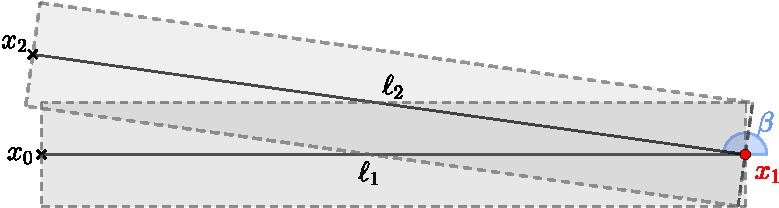
\includegraphics[width=.45\textwidth]{2D-1stOrderApproximation_rectangles_largeTA_largel2_nolabels-crop}}\hfill
	\subfloat[{Case 2: A large turning-angle with small $\ell_2$}]{%
		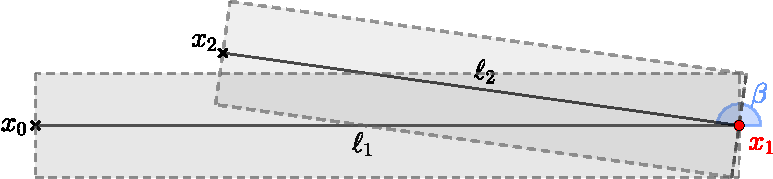
\includegraphics[width=.45\textwidth]{2D-1stOrderApproximation_rectangles_largeTA_smalll2_nolabels-crop}}\\
	\subfloat[Case 3: A medium turning-angle]{%
		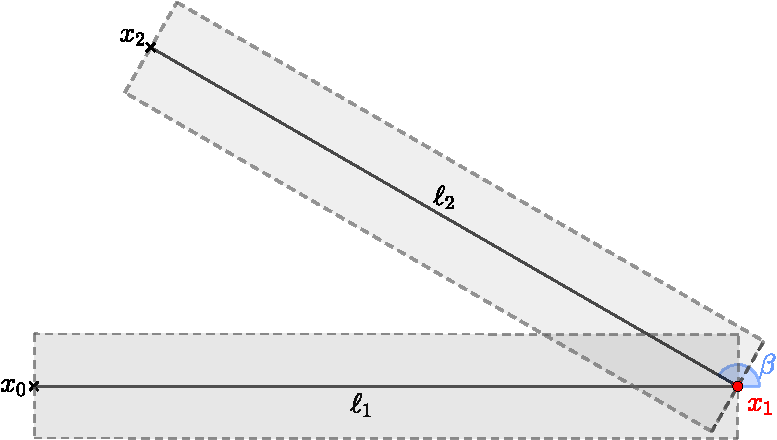
\includegraphics[width=.5\textwidth]{2D-1stOrderApproximation_rectangles_mediumTA_nolabels-crop}}\hfill
	\subfloat[Case 4: A small turning-angle]{%
		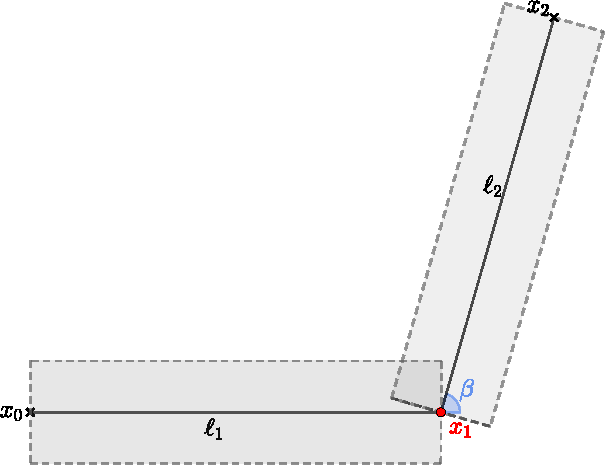
\includegraphics[width=.5\textwidth]{2D-1stOrderApproximation_rectangles_smallTA_nolabels-crop}}
	\caption[The four different cases for the turning-angle that we consider when determining the area of overlap]{The four cases that need to be considered to determine the overlapping area between two steps, with different turning-angles giving rise to different cases. When the turning-angle is large, which of case $1$ or case $2$ arise depends on the relative sizes of $\ell_1$ and $\ell_2$. When $\ell_2$ is sufficiently small, case $3$ becomes case $2$. Four more cases exist for turning-angles greater than $\pi$, although these are mirrors of the four cases above.}\label{fig:2d_model:firstorder:fourcases}
\end{figure}

Throughout the derivation of the area, we are forced to make some further simplifications in order to be able to realistically solve the problems. For example, there is actually more than $4$ cases to consider, since there is a separate case in between case $1$ and case $2$, although this only occurs at very specific angles and is similar in size to both of these two, so we exclude this. There are also times where we assume that very small triangles of area are right-angled, or else the expressions for the area would be far more complicated for little difference in accuracy. We use Monte Carlo simulations in \cref{sec:2dmodel:simulations:MC_area} to ensure our expressions for the area are suitably accurate. 

Even with these simplifications, deriving expressions for the area covered by a step is quite tedious and results in complicated expressions. 
For this reason, we relegate the derivation of the first-order area to \cref{sec:2dmodel:1starea}.
The resulting expressions for the area of overlap between consecutive steps 
are
\begin{equation*}
A_{\text{overlap}} = 
\begin{cases}
r_v^2 \left|\tan(\beta/2)\right| \quad &\text{if } \beta \leq \pi/2 \text{ or } \beta \geq 3\pi/2,\\\\
\displaystyle \frac{r_v^2 \left|\sin(\beta)\right|}{1-\left|\cos(\beta) \right|} &\text{if } \pi/2  \leq \beta \leq  \pi-\arcsin\left( \frac{2r_v}{\min(\ell_1,\ell_2)} \right),\\
&\text{or }\pi+\arcsin\left( \frac{2r_v}{\min(\ell_1,\ell_2)} \right) \leq \beta \leq 3\pi/2\\\\
\displaystyle \frac{1}{2} \left[-\min(\ell_1,\ell_2)^2 \left|\tan(\beta)\right| \right. &\text{if }\pi-\arcsin\left( \frac{2r_v}{\min(\ell_1,\ell_2)} \right) \leq \beta\\
\left.+ 2r_v \min(\ell_1,\ell_2)(2+\tan^2(\beta))\right.  &\text{and } \beta \leq \pi +\arcsin\left( \frac{2r_v}{\min(\ell_1,\ell_2)} \right).\\
\left. - r_v^2 \left|\tan^3(\beta)\right| \right]   
\end{cases}
\end{equation*}

Then, the total area covered by a step of length $\ell_2$ with turning-angle $\beta$ and previous step-length $\ell_1$ is
\begin{equation}
\label{eq:2dmodel:1storder:area_analytic}
A = 2\ell_2 r_v - A_{\text{overlap}}.
\end{equation}


In \cref{sec:2dmodel:simulations:MC_area}, we use Monte Carlo simulations to show \cref{eq:2dmodel:1storder:area_analytic} is close to the true value of $A$.

\subsubsection{Probability density function of the new area covered}
Let $f_A(x)$ be the \ac{PDF} representing a forager taking a step that covers $x$ amount of new area. We can express this as
\begin{equation*}
f_A(x) = \int_{\ell_1=\lmin}^\infty \int_{\beta=0}^{2 \pi} f_A (x,\beta,\ell_1) d\beta d\ell_1,
\end{equation*}
where $\ell_1$ is the length of the forager's previous step, $\beta$ is the forager's turning angle, and $x$ is a function of $\ell_1$, $\ell_2$ and $\beta$. Since the turning angle and the length of a step are drawn independently, we can further rearrange this to get
\begin{equation}
\label{eq:2d_model:fa_conditional}
f_A(x) = \int_{\ell_1=\lmin}^\infty \int_{\beta=0}^{2 \pi} f_A(x \mid \beta,\ell_1) f_{TA}(\beta) f(\ell_1) d\beta d \ell_1,
\end{equation}
where $f_{TA}$ is the density of the forager's turning angle, and $f(\ell_1)$ is the \ac{PDF} of the forager's previous step. The area covered by a step is a piecewise function that depends on whether $\ell_1 < -\ell_2 \cos(\beta)$ or $\ell_1 \geq -\ell_2 \cos(\beta)$, so we could write it as two separate integrals:

\begin{multline*}
f_A(x) =  \int_{\ell_1=\lmin}^{\ell_2} \int_{\beta=0}^{2 \pi} f_A(x \mid \beta,\ell_1) f_{TA}(\beta) f(\ell_1)f(\ell_2) d\beta  d \ell_1\\
+ \int_{\ell_1=\ell_2}^\infty \int_{\beta=0}^{2 \pi} f_A(x \mid \beta,\ell_1) f_{TA}(\beta) f(\ell_1) f(\ell_2)d\beta  d \ell_1.
\end{multline*}

Then, we can further split up the integrals to get
\begin{multline*}
f_A(x) =  2 \int_{\ell_1=\lmin}^{\ell_2} \int_{\beta=0}^{\pi/2} f_A(x \mid \beta,\ell_1) f_{TA}(\beta) f(\ell_1) d\beta d \ell_1\\
+  2\int_{\ell_1=\lmin}^{\ell_2} \int_{\beta=\pi/2}^{\pi - \arcsin(2r_v/\ell_1)} f_A(x \mid \beta,\ell_1) f_{TA}(\beta) f(\ell_1)d\beta  d \ell_1\\
+  2 \int_{\ell_1=\lmin}^{\ell_2} \int_{\beta=\pi - \arcsin(2r_v/\ell_1)}^{\pi} f_A(x \mid \beta,\ell_1) f_{TA}(\beta) f(\ell_1) d\beta  d \ell_1\\
+2 \int_{\ell_1=\ell_2}^\infty \int_{\beta=0}^{\pi/2} f_A(x \mid \beta,\ell_1) f_{TA}(\beta) f(\ell_1) d\beta d \ell_1\\
+2\int_{\ell_1=\ell_2}^\infty\int_{\beta=\pi/2}^{\pi-\arcsin(2r_v/\ell_2)} f_A(x \mid \beta,\ell_1) f_{TA}(\beta) f(\ell_1) d\beta  d \ell_1\\
+2\int_{\ell_1=\ell_2}^\infty \int_{\beta=\pi-\arcsin(2r_v/\ell_2)}^{\pi} f_A(x \mid \beta,\ell_1) f_{TA}(\beta) f(\ell_1) d\beta d \ell_1,
\end{multline*}
where we have $6$ rather than $12$ different terms since we have multiplied each term by $2$ due to symmetry.
For the first term, note that $f_A(x \mid \beta, \ell_1) = 2r_v \ell_1 - r_v^2 \tan(\beta/2)$ by \cref{eq:2dmodel:1storder:area_analytic}. We can rearrange this expression to find the inverse
\[x = 2r_v \ell_2 - r_v^2 \tan(\beta/2) \implies \ell_2 = \frac{x+r_v^2 \tan(\beta/2)}{2r_v}.\]
Thus, we can replace $f_A(x \mid \beta, \ell_1)$ with $f \left(\frac{x+r_v^2 \tan(\beta/2)}{2r_v}\right)$.
We can do similarly for the other integrals.
However, note that the third and the sixth integrals have an expression for $A$ which cannot be inverted easily, meaning we must either make further simplifications or solve the integrals numerically.



After solving for $f_A(a)$, we then must substitute the result, along with our piecewise function $A$ into
\begin{equation*}
\Pr(\text{not found}) = \int_{A_{\min}}^\infty e^{-a\rho} f_A(a)da,
\end{equation*}
which is then used to find $\E{N}$. For the first-order model, every step except the first step has the same probability of finding food, and so if we account for this we can also consider $\tau$ as a geometric random variable.
We do not proceed any further with this process analytically since the remainder of the work is dependent on the choice of step-length distribution, as well as requiring integration over complicated expressions.

\subsubsection{Truncated step-length}

As with the zeroth-order model, we need to determine the expected truncated length of a step, given the forager was intending to step a distance $\ell$. 
However, in the first-order model this will depend on the size of the steps as well as the turning-angle and the radius of vision. 
The probability of finding a target depends on the amount of new area being searched, and so should depend heavily on the geometry formed by the current and previous step.
Recall that our expression for $A$, \cref{eq:2dmodel:1storder:area_analytic}, required that $\ell_2 \geq r_v$, meaning we do not have a valid expression for the amount of new area covered while the forager is travelling the first $r_v$ distance.
We can assume that these values are also valid for the first $r_v$ distance of a step, although this is shown to be fairly inaccurate in \cref{sec:2dmodel:simulations}.
This assumption would allow us to write down some integrals for the truncated step-length, though we would not be able to solve them.

\subsubsection{Efficiency}

Although we have not been able to solve the first-order model analytically, we can draw some conclusions from the expressions we have found. Consider first the case when $\ell_1 < \ell_2$. The first two intervals for the area of overlap, for small and medium angles, have no dependence on $\ell_1$ or $\ell_2$, apart from changing when an angle is considered large. The area of overlap in the final interval, for large angles, will depend on the length of the previous step, $\ell_1$, since it is the smaller of the two steps. Thus, once $\ell_2$ gets larger than $\ell_1$, the area of overlap does not change. The total amount of new area will still increase as $2r_v\ell_2$. When $\ell_2 \leq \ell_1$, the total amount of overlapping area is similar for small and medium angles. The amount of overlapping area for large angles is very large, and increases as $\ell_2$ increases. Thus, we can conclude that to maximise the amount of new area covered, a forager should take steps as large as possible, regardless of what the previous step was. This would correspond to, for example, an exponential distribution with $\mu \to 0$ or a power-law distribution with $\mu \to 1$, which matches known results for destructive foraging.


\section{Simulations}
\label{sec:2dmodel:simulations}
\subsection{Monte Carlo simulations for the first-order area}
\label{sec:2dmodel:simulations:MC_area}
We use Monte Carlo simulations to estimate the true value of $A$, and compare with the results of our analytic expression. We first define the rectangle of search area from the previous step, at the following points in clockwise order: $(-\ell_1,r_v)$, $(0,r_v)$, $(0,-r_v)$, and $(-\ell_1,-r_v)$. Then,we can generate points in the area of the second step to determine the area of overlap. For some fixed $\ell_2$ and turning-angle $\beta$, we choose a uniformly distributed random variable $u_1$, between $0$ and $\ell_2$, and can then define the point $(u_1 \cos(\beta),u_1 \sin(\beta))$. This point is some random point along the path of the forager's current step. Next, we randomly generate a uniformly distributed random variable $u_2$, between $-r_v$ and $r_v$, to represent any point along the perpendicular radius of vision. Thus, the final location of our point will be at $\left(u_1 \cos(\beta)+u_2\sin(\beta), u_1 \sin(\beta) - u_2 \cos(\beta)\right)$.

If the randomly generated point is within the rectangle of the previous step, it is overlapping with the previous step. We randomly generate $50000$ points using the above process, and can estimate the proportion of overlapping points as $n/50000$, where $n$ is the number of points that were overlapping. The total area of overlap will therefore be, $(n/50000) 2 r_v \ell_2$, and so the newly explored area is $A=2(50000-n)/n r_v \ell_2$. We take the Monte Carlo simulation to be the true value, and determine the relative error of the analytic expressions based on this. Implicit in this is the assumption that the Monte Carlo simulations produce the exact value for the area, which is not true, although relative to the error in our analytic expressions the Monte Carlo simulations produce very accurate values. \Cref{fig:OverlappingArea_example} shows an example of this. We repeat this whole process for various values of $\ell_1$, $\ell_2$, $r_v$, and $\beta$, and compare the found area of overlap with our analytic expressions \cref{eq:2dmodel:1storder:area_analytic}.

\begin{figure}[h!]
	\centering
	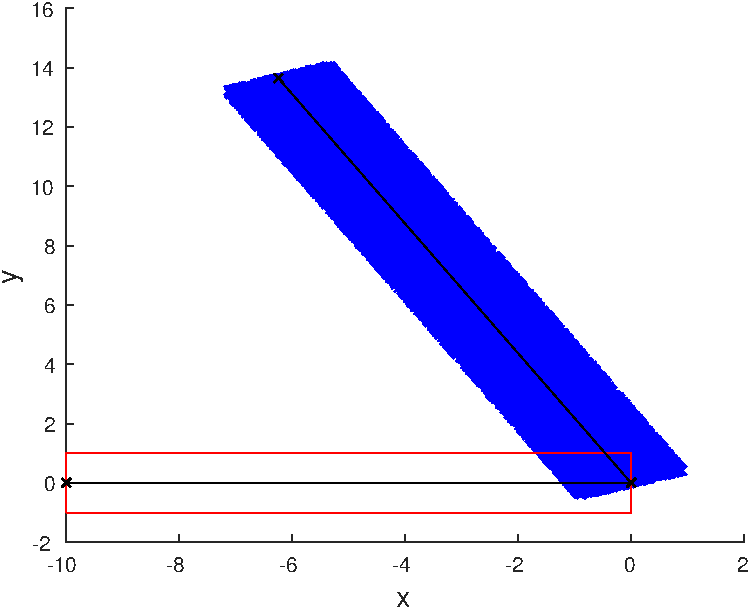
\includegraphics[scale=0.73]{OverlappingArea_10l1_15l2_1rv_2beta_50000reps}
	\caption[An example step where the overlapping area is approximated using a Monte Carlo simulation, and compared with our analytic expressions]{An example of our Monte Carlo simulation method to determine the amount of overlapping area between two consecutive steps, for $\ell_1=10$, $\ell_2 = 15$, $r_v=1$, and $\beta=2$. The area covered by the previous step is represented by the red rectangle, and each of the $50000$ simulated points are blue crosses. In this case, $n=243$ points overlap with the red rectangle, and the full area of the current step is $2r_v\ell_2 = 30$, so the area of overlap is $A=1.458$. The amount of total new area covered is $A=28.542$ according to this method, and $A=28.443$ according to our analytic approximation, giving a relative error of $0.0072$. \label{fig:OverlappingArea_example}}
\end{figure}

\begin{figure}[h!]
	\centering
	\subfloat[{Relative error vs. turning-angle $\beta$}]{%
		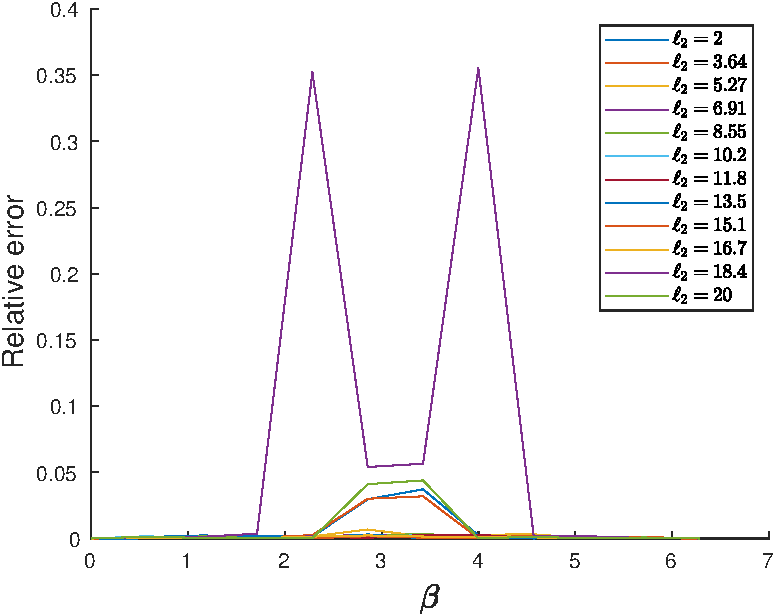
\includegraphics[width=.50\textwidth]{OverlappingArea_eVsbeta_10l1_1rv_50000reps}\label{fig:OverlappingArea_beta}}\hfill
	\subfloat[{Relative error vs step-length $\ell_2$}]{%
		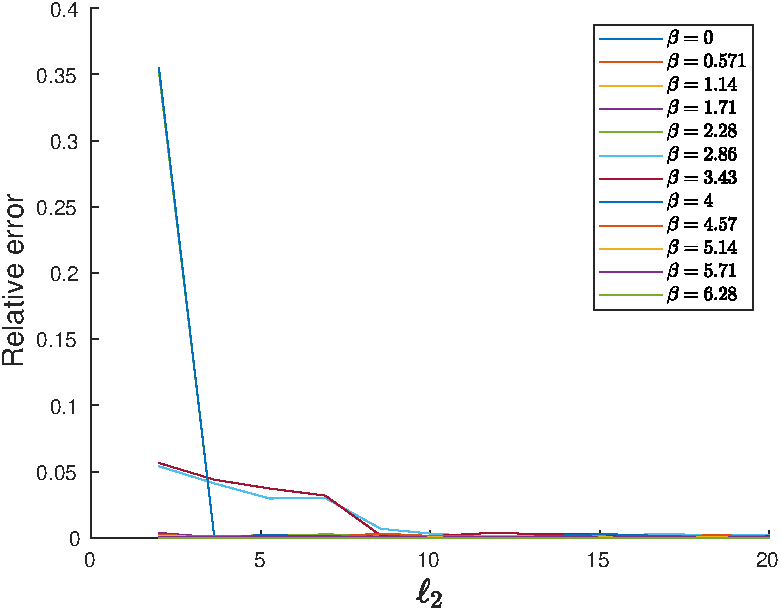
\includegraphics[width=.50\textwidth]{OverlappingArea_eVsl2_10l1_1rv_50000reps}\label{fig:OverlappingArea_l2}}\\
	\caption[The relative error in our analytic expressions for the overlap plotted against the step-length and the turning-angle]{The relative error plotted against the step-length $\ell_2$, for $2 \leq \ell_2 \leq 20$ at $10$ equispaced intervals and against the turning-angle $\beta$, for $0 \leq \beta \leq 2 \pi$.  The radius of vision is $r_v=1$ and $\ell_1 = 10$. Large relative errors occur at $\beta=2.86$ and $\beta=4$ take large values for small values of $\ell_2$, and all other values of $\ell_2$ and $\beta$ produce a relative error less than $0.065$.}\label{fig:OverlappingArea}
\end{figure}

Looking first at \cref{fig:OverlappingArea_beta}, we see that the relative error in the area is less than $0.05$ everywhere except for when $\ell_2 = 2$. When $\ell_2=2$, there are two large spikes in the relative error when $\beta = \approx 2.2$ and $\beta \approx 4.1$. The reason for the large error at these points are the assumption we made in \cref{app:area}, that $\ell_2 \gg r_v$, and $\ell_1 \approx \ell_2$, both of which are violated at these values, causing the wrong piecewise expression to be considered. This happens for these angles specifically because they are normally close to a threshold angle. Also looking at \cref{fig:OverlappingArea_l2}, we can draw the same conclusions, with a lower $\ell_2$ causing larger errors, as well as large errors occurring at $\beta = 0$, $\beta\approx 2.86$, and $\beta \approx 4.57$.

\begin{figure}[h!]
	\centering
	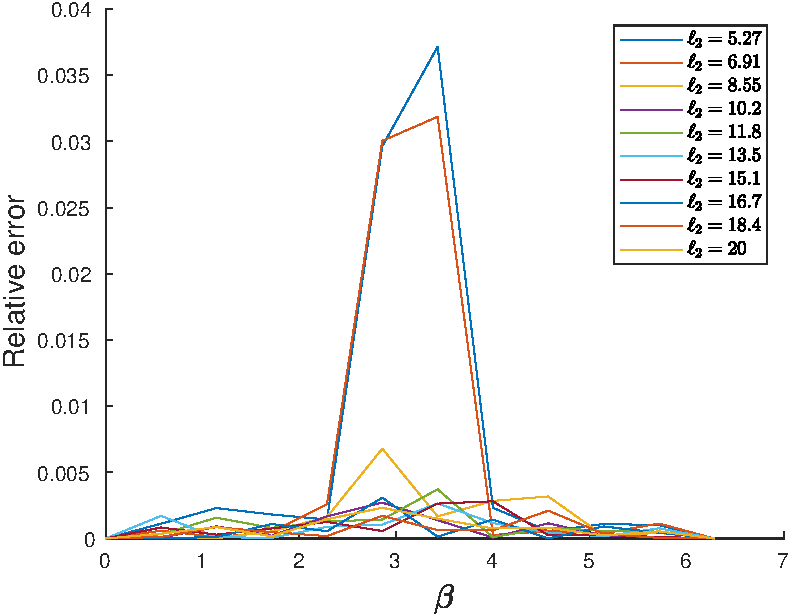
\includegraphics[scale=0.68]{OverlappingArea_eVsbeta_10l1_1rv_50000reps_skip2}
	\caption[The relative error in our analytic expressions for the overlap plotted against the turning-angle]{The relative error plotted against the turning angle $\beta$, for $0 \leq \beta \leq 2 \pi$ at $10$ equispaced intervals. The radius of vision is $r_v=1$ and $\ell_1 = 10$, and lines are plotted for $10$ different values of $\ell_2$, from $5.27$ to $20$. The lines for $\ell_2=5.27$ and $\ell_2 = 6.91$ has large peaks near the centre, for values of $\beta$ near $\pi$, corresponding to a large turning angle, and all other values of $\ell_2$ and $\beta$ produce a relative error less than $0.05$. \label{fig:OverlappingArea_beta_skip}}
\end{figure}

In \cref{fig:OverlappingArea_beta_skip} we plot the relative efficiency against the turning-angle as we did in \cref{fig:OverlappingArea_beta}, except we exclude the lowest two values of $\ell_2$. Now, the two lowest values of $\ell_2 = 5.27$ and $\ell_2=6.91$ produce the largest error, at $\beta \approx \pi$. The error at these points is less than $0.04$, and the cause for the error is the approximations made for the case of large turning-angles (case $1$) in \cref{app:area}. For all other values of $\beta$ and $\ell_2$, the relative error is lower than $0.01$, which is a good level of accuracy.

In summary, the analytic expressions from \cref{eq:2dmodel:1storder:area_analytic} are relatively accurate for most values of $\beta$ and $\ell_2$, with some larger errors occurring when $\ell_2$ is small and $\beta \approx \pi$. The effect that these points of inaccuracy will have on the overall calculation will depend on the turning-angle distribution as well as the step-length distribution. For example, a step-length distribution with a very large minimum step-size would always produce large steps and would not suffer from many of these inaccuracies. 


\FloatBarrier
\subsection{Simulating our two-dimensional model}
\label{sec:2dmodel:simulation}

We use Matlab to simulate the model outlined above. We initially use a $50 \times 50$ search space, and generate food targets according to a spatial Poisson point process on this search space, with density $\rho$. We simulate the Poisson process by first drawing a number $N \sim \mathcal{P}(50^2\rho )$, and then drawing $N$ random variables from $x \sim \text{Uni}[0,50]$ and $N$ random variables from $y \sim \text{Uni}[0,50]$, and pairing these up to form the coordinates of the targets.

The forager begins at the centre of the search space at $(25,25)$. To simulate the movement of the forager, we draw an angle with $\theta \sim \text{Uni}[0,2\pi]$ and a step-length from our step-length distribution using inverse transform sampling. Thus, we are able to simulate a series of coordinates corresponding to the foragers steps. When a forager steps outside of the search area, we extend the search area in multiples of $50$ until the foragers new location is within the search area, and generate new targets in the new area in the same way as above.

After each step is taken, we check to see if a target has been located. To do this, we determine the perpendicular distance that each food patch is away from the line segment connecting the start and end points of a step. If we wanted to consider the circle of vision at the start and end of each step, we could also check the distance each point is from these points, in any direction. However, for consistency with our analytic model we exclude these. If any of these distances are less than $r_v$, then a target is located on that step. The located target is the one that is closest to the starting point of the step.

\Cref{fig:TwoDForager_Exponential} shows a single simulation of our model, with the forager using an exponential distribution. This model currently corresponds to the infinite order foraging model since once an area has been explored unsuccessfully, there is no chance of finding points there when reexploring the area. To instead consider our zeroth-order approximation, each time a step fails to locate food we generate targets according to a Poisson distribution as done above, although this time only in the area that was just explored. For the first-order model, we also do this although there is a lag of $1$ step before each regeneration. We can then consider any $k$th-order approximation by setting the regeneration lag to $k$.

\begin{figure}[h!]
	\centering
	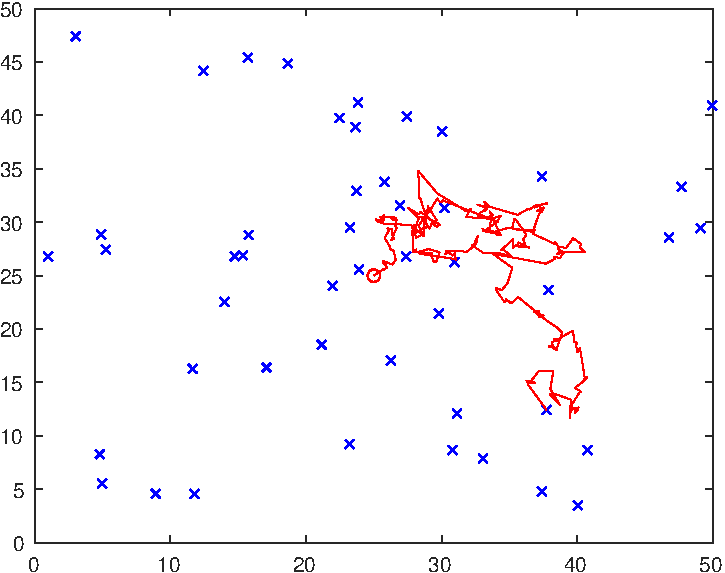
\includegraphics[scale=0.68]{TwoDForager_Exponential_0lmin_1-80mu_0-20rv_0-02rho}
	\caption[An example simulation of our two-dimensional]{A simulation of our two-dimensional foraging model, with parameters $r_v=0.2$, $\rho=0.02$. The forager takes steps from an exponential distribution with $\lmin=0$ and $\mu = 1.8$. No points are regenerated in areas that have already been explored, and thus this corresponds to the infinite order model. \label{fig:TwoDForager_Exponential}}
\end{figure}

\Cref{fig:TwoDForager_Efficiency_PowerLaw} compares the average step-length, mean number of steps, and efficiency, respectively, for the zeroth-order, first-order and infinite order models for a power-law forager. The efficiency of the simulated zeroth-order model matches the exact expression for the efficiency that we found, \cref{eq:2dmodel:0th:efficiency}. The efficiency of the first-order model decreases slightly as $\mu$ increases, and is slightly less efficient than the zeroth-order model, which is to be expected since targets are not being regenerated as quickly. The decrease in efficiency as $\mu$ increases also matches our conclusions from the analytic work on the first-order model, where we reasoned that the larger each step was, the less backtracking that would occur and hence more fresh area would be explored. Also, we are considering destructive foraging, for which it is known that ballistic motion offers the best efficiency (e.g. \cite{Viswanathan_1999}). 

The efficiency of the infinite order model decreases much faster than either the zeroth or first-order models. 
While the zeroth and first-order model seem to be fairly similar to each other, the infinite order model is significantly different to both, indicating that neither the zeroth or first-order models are accurate approximations for the infinite order model, and higher order models are needed. However, the first-order model is already too complicated to fully solve analytically, so an analytic approach to even higher order models is out of the question. Nonetheless, the zeroth-order and the first-order models can be considered as upper bounds for the infinite-order model. 


\begin{figure}[h!]
	\centering
	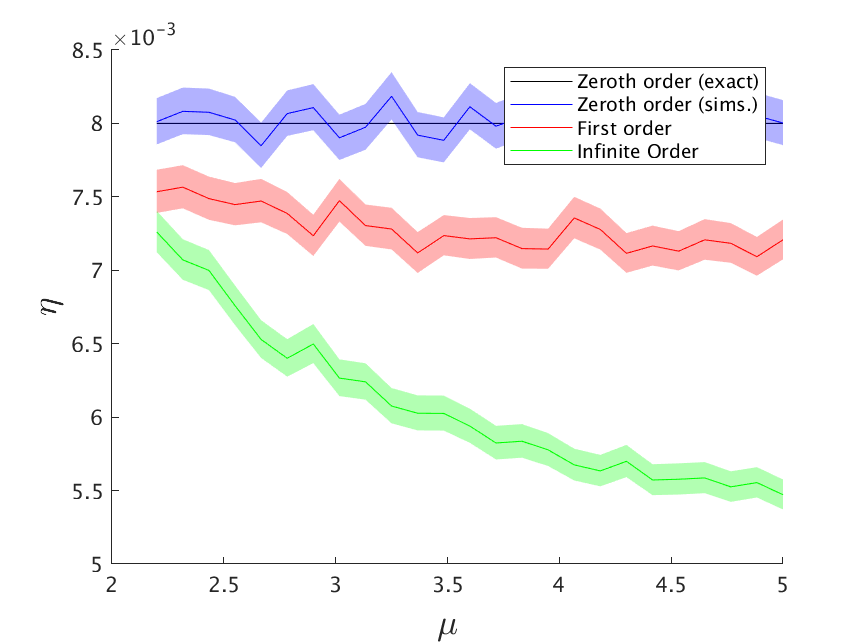
\includegraphics[scale=0.68]{TwoDForager_Efficiency_PowerLaw_1lmin_0-20rv_0-02rho_10000reps}
	\caption[Comparison of zeroth-order, first-order, and infinite-order model, and the analytic results for the zeroth-order]{The mean efficiency for the zeroth, first, and infinite order models with 95\% confidence intervals, as well as the exact result found for the zeroth-order model. The forager takes steps from a power-law distribution with $\lmin=1$, and for $25$ equispaced values of $\mu$ between $2.2$ and $5$. The mean is taken over $10000$ repetitions. \label{fig:TwoDForager_Efficiency_PowerLaw}}
\end{figure}